\documentclass[cclicense]{hmcthesis}

\usepackage{util}
\usepackage{math}

\usepackage{extarrows}
\usepackage{kbordermatrix}

\usepackage{makeidx}
\makeindex

\newcommand*{\x}[1]{\ensuremath{X^{(#1)}}}
\providecommand*{\xs}{\mathcal X}
\providecommand*{\ms}{\mathcal M}
\providecommand*{\ns}{\mathcal N}
\providecommand*{\N}{\mathbb{N}}
\newcommand*{\vbar}{\;\big\vert\;}
\newcommand*{\STB}{\::}
\DeclareMathOperator*{\argmax}{arg\ max}

\newcommand*{\mle}{\mathrm{mle}}
\newcommand*{\emp}{\mathrm{emp}}

\numberwithin{equation}{chapter}
\numberwithin{thmcounter}{chapter}

\title{Algebraic Methods for Log-Linear Models}
\author{Aaron Pribadi}
\thesisyear{2012}
\advisor{Michael Orrison}
\reader{Weiqing Gu}

\begin{document}

\frontmatter

\maketitle

\tableofcontents



\chapter{Abstract}
    This will be an abstract.

\chapter{Acknowledgements}
    There will be acknowledgements.

\mainmatter

\chapter{Introduction}

    Discrete observations model the world in almost the simplest way possible.
    Things are labelled and put them into categories: ``This ice cream is green
    and has sprinkles.''  Given enough observations, one can begin to make
    predictions.
    
    On the surface this procedure appears to be quite simple, but a deep well of
    difficult problems of intensely practical importance lies beneath.  The
    pervasive introduction of digital storage and computation has only increased
    the flood of data readily available.  In many cases, we cannot use the data
    as well as we would like.  Problems surrounding
    \begin{itemize}\noparspace
    \item genomic sequences,
    \item image recognition,
    \item natural language processing
    \item voting data,
    \item product recommendation,
    \end{itemize}
    and so on are active areas of research driven by real-world concerns.

    Questions arising from the analysis of discrete data pose many challenges,
    but at the same time offer rich mathematical structures.  One hope is that
    ideas from `pure' mathematics, particularly geometry and algebra, can offer
    guiding principles and effective techniques for the analysis of data.
    Another hope is that the avenues suggested by the needs of practical
    problems will be of intrinsic mathematical interest.
    
    We examine log-linear models, a type which interacts especially well with
    ideas from geometry and algebra.  Even though log-linear models conform to a
    rigid format, many standard techniques from the analysis of discrete data
    fall under its umbrella.  As is often the case, the presence of a linear
    structure in such models offers a shortcut to tractability.  The linear
    structure furthermore allows concerns of symmetry and invariance to be more
    readily exploited.  Within this framework, algebraic ideas can be brought to
    bear on model selection.

    We pay special attention to models on the sample space $\{0, 1\}^n$ of
    binary strings of a fixed length.  In some sense, this space is the most
    straightforward way to encode finite data compactly.  This sample space also
    has a large amount of symmetry, and is a homogeneous space with respect to
    its natural automorphism group.  We introduce a general parametrization for
    log-linear models on a finite homogeneous space $\xs$ for which the
    representation $L(\xs)$ is multiplicity-free.  This parametrization respects
    the isotypic decomposition of $L(\xs)$.  We then construct this
    parametrization explicitly for the case $\xs = \{0, 1\}^n$.  Such a
    parametrization is one of several for $\{0, 1\}^n$, and may offer certain
    advantages over other options when used in algorithms for finding sparse
    models.

\chapter{Discrete Models}

    \section{Discrete Data}

    A random variable (from an elementary standpoint) is either 
    \begin{itemize}\noparspace
    \item discrete, when its sample space is countable, or
    \item continuous, when its sample space is a subset of $\R^n$.
    \end{itemize}
    We consider the first case.  In particular, we usually take the relevant
    sample space to be finite.  Because we can then deal with
    finite-dimensional spaces, this assumption simplifies many ideas.

    Another fundamental assumption is that repeated observations are independent and
    identically distributed random variables.  That is, the observations $\x 1,
    \ldots, \x m$ are random variables, and each is distributed according to the
    same underlying probability distribution, $\x i \sim p$.  Given an observed
    set of values for the $\x i$, a basic objective is to estimate the
    underlying probability distribution $p$.

    Let each $\x i$ take an observed value from the finite sample space $\xs$.
    Because the order of the observations does not matter, we can summarize the
    series of observations with the counts
    \begin{equation*}
        u(x) = \pdel{\text{the number of $i$ for which $\x i = x$}}
    \end{equation*}
    for $x \in \xs$.  If the number of possible outcomes $|\xs|$ is small
    relative to the number of samples $m$, then the empirical distribution
    \begin{equation}
        p_\emp(x) = \frac{u(x)}{m}
        \label{eq:empirical}
    \end{equation}
    is a useful estimate of the true distribution $\x i \sim p$.

    It is sometimes the case that $|\xs|$ is very large.  Without a
    correspondingly large number of samples, the empirical distribution $p_\emp$
    may not adequately capture the underlying distribution $p$.  Such sample
    spaces arise naturally in a variety of situations, especially when
    combinatorial processes are involved.
    \begin{itemize}
    \item Multivariate data occurs when multiple things are observed at once.
    The sample space is a cartesian product
    \[
        \xs = \xs_1 \times \cdots \times \xs_k
    \]
    of several finite sets.  If $k$ labels are assigned to an observation, then
    the component space $\xs_i$ could be the set of possible values for the
    $i$th label.  For example, a person can have an eye color, a handedness, a
    gender, a political affiliation, and many more characteristics. In that
    case, $\xs_1$ would be a set of colors, et cetera.
    
    If each variate has approximately the same number of possible values, then
    the size of the sample space is exponential in the number of variates.  

    A comprehensive reference for the statistical analysis of multivariate data
    is the book by \citet{DMA}.

    \item Group-valued data occurs when discussing arrangements of a system.
    For example, voters in an election could be asked to rank $n$ candidates.
    The sample space is then the symmetric group $\xs = S_n$.  Clearly, it is
    rather easy to construct simple examples with large numbers of possible
    outcomes, e.g. $n!$ for the symmetric group.
    
    When there is no `special' base point of the sample space to call the
    identity of the group, another choice is to consider the sample space as a
    homogeneous space.

    \end{itemize}
    For the empirical distribution to produce a good estimate of the underlying
    distribution, a prohibitively large number of samples is required.

    In order to analyze data with a large number of states, it is often fruitful
    to restrict which distributions we consider.  Ideally, we would use the
    structure of the underlying sample space in order to better analyze data.

    \begin{example}[Binary Multivariate Data]
        The UCI database contains a large number of data sets useful for the
        evaluation of machine learning techniques \citep{UCIData}.  The
        Congressional Voting Records data set contains Congressional voting
        records on a number of key issues.
        \begin{figure}[H]
            \centering
            \begin{verbatim}
            1) democrat   n y y n y y n n n n n n y y y y
            2) republican n y n y y y n n n n n y y y n y
            3) democrat   y y y n n n y y y n y n n n y y
            4) democrat   y y y n n n y y y n n n n n y y
            5) democrat   y n y n n n y y y y n n n n y y
            \end{verbatim}
            \vspace{-1.5\baselineskip}
            \caption{A few lines from the Congressional Voting Records
            data set.}
        \end{figure}
        \noindent For this data set, each variate has two possible values,
        either the set $\{\texttt{yes}, \texttt{no}\}$ or $\{\texttt{democrat},
        \texttt{republican}\}$.  (This ignores missing values, e.g.  where a
        representative did not vote.)  The sample space may be written as $\xs =
        \{0, 1\}^7$, the set of binary strings with 7 bits.  
        
        In this example, the size of the sample space is quite large, $\|xs| =
        2^{17} = 131072$.  There are $435$ samples in the data set.  In order to
        make sense of the data, some assumptions about potential distributions
        are needed.  One possible assumption is that each variate is independent
        from the others.  This, however, would be perhaps too simplistic.
        \label{ex:binary-voting}
    \end{example}


    \section{The Simplex and Statistical Models}

    We take a geometric view of statistical models.  The formulation of
    statistical objects in terms borrowed from other parts of mathematics allows
    statistical problems to be attacked with a large range of useful tools.  The
    adoption of this perspective is in large part influenced by the lecture
    notes by \citet{DSS08}, which summarize recent progress in using the tools
    of algebraic geometry for statistics.

    A probability distribution on a finite set $\xs$ can be thought of as a
    real-valued function $p \in L(\xs)$ subject to the restrictions that
    $\sum_{x\in \xs} p(x) = 1$ and that $p(x) \ge 0$ for all $x \in \xs$.  The
    function $p$ is the probability mass function.  Finite sets are particularly
    convenient because we can always work with a probability mass function, and
    because the probability mass function is always embedded in an ambient
    finite dimensional vector space.  The space of all distributions on $\xs$ is
    a geometric object.
    
    \begin{definition} 
        \index{simplex}
        The \emph{standard simplex} of dimension $n$ is the subset
        \[
            \Delta_n = 
            \left\{(p_1, \ldots, p_{n+1}) \in \R^{n+1} \vbar 
            \sum_{i=1}^{n+1} p_i= 1, p_i \ge 0 \right\} 
        \]
        of $\R^{n+1}$.  If the appropriate dimension is either clear in context
        or irrelevant, then we may write $\Delta$, omitting the subscript.
    \end{definition}

    The simplex is a generalization of an equilateral triangle.  Low-dimensional
    simplices are familiar shapes; $\Delta_0$ is a point, $\Delta_1$ is a line
    segment, $\Delta_2$ is a triangle, and $\Delta_3$ is a tetrahedron.

    \begin{figure}[H]
        \centering
        \includegraphics[scale=1]{2-simplex.pdf}
        \caption{The 2-simplex.}
    \end{figure}

    There is a one-to-one correspondence between probability distributions on
    the set $\xs = \{x_1, \ldots, x_{n+1}\}$ and points in the simplex
    $\Delta_n$; the probability $p(i)$ is equal to the value of the coordinate
    $p_i$.  We therefore identify the two concepts with each other.
    Because the space of all probability distributions is a geometric
    object, it is easy to talk about specific families of probability
    distributions.

    \begin{definition}
    A \emph{statistical model} is a subset $\ms \subset \Delta$ of the
    probability simplex.  A \emph{parametrized model} $\ms$ with parameter space
    $\Theta$ is specified by a surjective map $\Theta \to \ms$.  We usually
    write $p_\theta$, with $\theta \in \Theta$, to denote a distribution from a
    parametrized model.
    \end{definition}

    Many statistical models have been studied and employed for the analysis of
    data, and the selection of an appropriate model is a delicate question.  In
    Section~\ref{sec:linear-models} we introduce a family of models with
    convenient properties.

    In an ideal situation, there is a hypothesis for an underlying mechanism
    producing the observable results.  In that case, a particular choice of
    model is easy to justify.

    \begin{example}[Binomial Model]

        The distribution $\mathrm{Binom}(N, \alpha)$ models the number of heads
        produced by $N$ independent `coin tosses', where \mbox{$0 \le \alpha \le
        1$} is the probability that a single toss produces a head.  It is
        defined by the probability density function
        \[
            p_\alpha(k) = {N \choose k} \alpha^k(1-\alpha)^{n-k}.
        \]
        for $k \in \{0, \ldots, N\}$.  The map $\alpha \mapsto p_\alpha$
        determines a parametrized statistical model.  The statistical model is a
        curve, i.e. a one-dimensional subset of the simplex.  

        The model $\mathrm{Binom}(2, \alpha)$ simulates two coin flips.  The
        three coordinates of a point in the model measure the probabilities that
        zero, one, and two heads will occur, respectively.

        \begin{figure}[H]
            \centering
            \vspace*{-0.2cm}
            \scalebox{1}{ \includegraphics[scale=0.7]{images/binomial.pdf} }
            \vspace*{-0.5cm}
            \caption{The binomial model for $N=2$. Make this 3-D?}
            \label{fig:binomial}
        \end{figure}

        \noindent As the parameter $\alpha$ varies over $[0,1]$, the statistical
        model traces out the curve 
        \[
            \alpha \longmapsto \big((1-\alpha)^2, 2\alpha(1-\alpha), \alpha^2\big)
        \]
        in the simplex $\Delta_2$ (see Figure~\ref{fig:binomial}).  

        If we knew that a coin was being flipped twice and did not know the
        odds of the coin, then the model $\alpha \mapsto \mathrm{Binom}(N,
        \alpha)$ would be an appropriate choice for the situation.
    \end{example}

    \begin{example}[Multivariate Independence]
        The independence model on a sample space $\xs = \xs_1 \times \cdots
        \times \xs_k$ assumes that each variate is independent.  For a
        distribution $p$ on $\xs$, the variates are said to be independent if
        $p$ factors as
        \[
            p(x) = p_1(x) \cdots p_k(x)
            \qquad
            \text{where}
            \qquad
            p_i(x) = \sum_{y_i = x_i} p(y) % \stackrel{y \in \xs}{x_i = y_i}} p(y)
        \]
        for all $x = (x_1, \ldots, x_k) \in \xs$.  Each factor $p_i(x)$ is a
        function only of the $i$th component of $x$.  Despite this simplistic
        assumption, the independence model is surprisingly effective in many
        situations, e.g. for naive Bayes classifiers.  
        
        The map 
        \begin{align*}
        \Delta_{|\xs_1|-1} \times \cdots \Delta_{|\xs_k|-1} 
        &\to \Delta_{|\xs| - 1} \\
        (p_1, \ldots, p_k) &\mapsto p_1 \cdots p_k
        \end{align*}
        gives a one-to-one parametrization of the independence model.  Counting
        dimensions indicates that the independence model imposes strict
        limitations on potential distributions.  The parameter space has
        dimension
        \[
            \dim 
            (\Delta_{|\xs_1|-1} \times \cdots \Delta_{|\xs_k|-1})
            =
            |\xs_1| + \cdots + |\xs_k| - k
        \]
        whereas the space of all distributions on $\xs$ has dimension 
        \[
            \dim(\Delta_{|\xs| - 1})
            =
            |\xs_1| \cdots |\xs_k| - 1.
        \]
        If the variates are binary, as in Example~\ref{ex:binary-voting}, then the
        model has dimension $k$ and the whole simplex has dimension $2^k - 1$.
        The latter grows much more rapidly with increasing $k$ than the former.
        \label{ex:independence1}
    \end{example}
    
\section{Likelihood and Model Complexity}
    In the analysis of data, there is a tension between how well an explanation
    fits the observed data, and how well such an explanation can be expected to
    generalize to new data.  While we do not explore all nuances of this
    trade-off, we do introduce a few fundamental concepts.

    One way to measure how well a distribution matches data is to ask the
    question, ``How likely is the data, given the distribution?''  A maximum
    likelihood estimate quantifies whether a model contains distributions
    suitable in that way.

    Let $\ms = \{p_\theta : \theta \in \Theta\}$ be a parametrized statistical
    model.  Suppose that some data $Z = \{z_1, \ldots, z_m\}$ are observed.  It
    is generally assumed that the data has been drawn from independent and
    identically distributed samples following an unknown true distribution from
    the model.
    
    \begin{definition}
    The \emph{likelihood function} of $\theta \in \Theta$ given the data $Z$ is
    \[
        L(\theta; Z) = \prod_{i=1}^n p_\theta(z_i).
    \]
    It is the probability that the observed data $Z$ would occur if the samples
    followed $p_\theta$.  Oftentimes, the \emph{negative log-likelihood}
    \begin{equation}
        -l(\theta; Z) = -\log L(\theta; Z) = -\sum_{i=1}^n \log p_\theta(z_i).
        \label{eq:negloglik}
    \end{equation}
    is used in lieu of the likelihood.  The negative log-likelihood is useful
    because the contributions to $-l(\theta; Z)$ from the observations $z_i$ are
    additive and each acts as a `penalty' or `loss'.
    \end{definition}
    \begin{definition}
    The \emph{maximum likelihood estimate} of the true parameter is the
    parameter 
    \[
        \theta_\mle = \argmax_{\theta \in \Theta} L(\theta; Z)
    \]
    that maximizes the likelihood of the data, or equivalently that minimizes
    the negative log-likelihood of the data.  In some cases, we identify the
    parameter $\theta$ with the distribution $p_\theta$. The term `maximum
    likelihood estimate' then refers to the distribution $p_\mle$ that maximizes
    the likelihood, given a choice of model.
    \end{definition}

    The fact that a maximum likelihood estimate might not exist or might not be
    unique is tacitly ignored.  Indeed $\{L(\theta; Z) \mid \theta \in \Theta\}$
    might be an open set, and the map $\theta \mapsto L(\theta; Z)$ might not be
    surjective.  In applications with real data, it is often the case that a
    precise maximum likelihood estimate is not necessary, and that an
    approximate value is sufficient.

    The distribution $p_\mle$ from the maximum likelihood estimate is the best
    one possible from the model.  Notice that if $\ms \subset \ns$ are two
    nested statistical models, then the maximal likelihood from $\ms$ is less
    than or equal to that from $\ns$.  Thus the size of the model determines how
    good of a distribution is possible.

    \begin{example}
        Suppose that the model does not restrict distributions at all, i.e.
        that the model is the whole simplex.  Then the maximum likelihood
        estimate is the empirical distribution $p_\emp$ as in
        \eqref{eq:empirical}.
    \end{example}

    \begin{example}[Multivariate Independence]
        Recall the independence model from Example~\ref{ex:independence1}.  The
        maximum likelihood estimate for the independence model is
        \[
            p_\mle(x) = \frac{u_1(x_1)}{m} \times \cdots \times \frac{u_k(x_k)}{m}
        \]
        where $x = (x_1, \ldots, x_k)$, $m$ is the number of samples, and
        $u_i(x_i)$ is the number of times that the $i$th variate of the
        observation is $x_i$.  In other words, we get a maximum likelihood
        estimate of each variate separately with its empirical distribution, and
        take the product distribution.
    \end{example}

    A larger model is deemed to contain more `complex' distributions.  The
    trade-off is that a larger model allows for probability distributions that
    fit the observed data better, but that might not generalize as well to
    subsequent observations.  This trade-off between model complexity and
    predictive power can be approached in a number of ways, and is explored in
    the standard literature.  Chapter 7 of the book by \citet{EOSL} is one
    reference.  
    
    There are at least two common methods to limit model complexity, which under
    certain circumstances produce the similar results.
    \begin{itemize}
    \item We can require that the estimated distribution $p$ is contained within
    some small model $\ms \subset \Delta$.
    \item We can minimize $-l(p) + \pi(p)$, i.e. the negative log-likelihood
    with an additional penalty term measuring the complexity of $p$.
    \end{itemize}
    Two criteria with complexity penalties are the Akaike information criterion
    and the Bayesian information criterion, defined
    \begin{align*}
        \mathrm{AIC} &= -2\,l(p_\mle) + 2d \\
        \mathrm{BIC} &= -2\,l(p_\mle) + (\log m) d
    \end{align*}
    where $-l(p_\mle)$ is the negative log-likelihood of the maximum likelihood
    estimate as in \eqref{eq:negloglik}, $d$ is the dimension of the parameter
    space $\Theta$, and $m$ is the number of samples.  These two criteria have
    different motivations, which are described in the above reference.  Notice,
    however, that the dimension of the model is used as the measure of its size.

\section{Log-Linear Models}
    \label{sec:linear-models}
    
    The selection of distributions can be treated as a problem in function
    estimation.  From the data we construct the empirical distribution \mbox{$p_\emp
    \in L(X)$}, and we wish to find another function $p \in L(X)$ that
    approximates $p_\emp$ subject to some set of restrictions.  
    
    The structure of $L(X)$ as a linear space suggests one method of
    approximation.  One can expand $p_\emp$ in terms of a basis $B = \{v_1,
    \ldots, v_n\}$ of $L(X)$, $p_\emp = \sum_{i=1}^n \lambda_i v_i$.  Any subset
    of the basis elements yields an approximation of $p_\emp$ from the
    projection to the subspace spanned by our subset.  One can select the terms
    with the largest coefficients $\lambda_i$, or, if the basis has some natural
    ordering, one can simply truncate the series.

    This method of approximation has at least one drawback, namely that negative
    probabilities are possible.  Dealing instead with log-probabilities is often
    fruitful.  In fact, log-linear models, i.e. discrete exponential families,
    are especially prevalent in the analysis of discrete multivariate data; see,
    for example, \citet{DMA}.
    \begin{definition}
        A \emph{log-linear} model $\ms_{V,h}$ is a statistical model of the form
        \[
            \ms_{V,h} = \cdel[\big]{p \in \Delta_{n-1} \:: \log p = (\log p_1, \ldots,
            \log p_n) \in V + h}
        \]
        where $h \in \R^n$, $V$ is a linear subspace of $\R^n$, and $V + h$ is
        an affine subspace.
    \end{definition}

    In many useful situations $h = 0$, so the log-linear model is associated
    with a vector subspace of $L(\xs)$.
    The usual definition of an exponential family (which need not be over a
    finite sample space) is as follows.
    \begin{definition}
        An \emph{exponential family} over a sample space $\xs$ parametrized by
        $\Theta$ contains distributions of the form
        \[
            p_\theta(x) = 
            \frac 1 {Z(\theta)}
            \exp\pdel*{
                \displaystyle \sum_{i=1}^d \eta_i(\theta)T_i(x) + h(x)
            }
        \]
        where $\eta : \Theta \to \R^d$, $T:\xs \to \R^d$, and $h: \xs \to \R$
        are known functions, and $Z:\Theta \to \R$ is a normalizing constant
        known as the partition function.
    \end{definition}
    An exponential family is a log-linear model when $\xs$ is finite and $\eta$
    is the identity map $\R^d \to \R^d$, as $p_\theta$ is constrained to lie in
    the affine space
    \[
        \mathrm{span}\cdel*{
            (T_i(x_1), \ldots, T_i(x_n)) \:: i \in \{1, \ldots, d\}
        } + h
    \]
    where $h$ is interpreted as a vector in $\R^n$.  

    \begin{example}[Binary Independence]
        The independence model with strictly positive probabilities is a
        log-linear model.  We compute this explicitly for the case where the
        sample space is $\xs = \{0, 1\}^2$.  One can verify that the two bits
        are independent for a distribution $p$ on $\xs$ if and only if 
        the row span of the matrix
        \[
            \kbordermatrix{
                & 00 & 01 & 10 & 11 \\
                &  1 &  1 &  0 &  0 \\
                &  0 &  0 &  1 &  1 \\
                &  1 &  0 &  1 &  0 \\
                &  0 &  1 &  0 &  1
            }
        \]
        contains $\log p$.  Notice that the matrix has rank 3, so that the
        independence model is a proper subset of the full simplex.
    \end{example}

    There is another form in which log-linear models are often presented.
    Define an `energy' function $H: \xs \to \R$.  The corresponding
    \emph{Boltzmann} distribution is defined
    \[
        p(x) = \frac 1 Z \exp(-H(x))
    \]
    where
    \[
        Z = \sum_{x \in \xs} \exp(-H(x))
    \]
    is a normalizing constant known as the partition function.  If the possible
    values for $H$ in a model are all linear combinations of some basis
    functions, then the model is log-linear.  This form is motivated by examples
    from statistical mechanics, where the probability of a state is proportional
    to $e^{-E/(k_BT)}$, where $E$ is the energy of the state, $T$ is the
    temperature, and $k_B$ is the Boltzmann constant.

\section{Sparsity and Regularization}
    \label{sec:regularization}

    Why are we so keen to cut down the number of dimensions?  The reason, which
    arises in optimization and statistics, is colorfully termed the \emph{curse
    of dimensionality}.  It is easiest to illustrate the problem in another
    closely related setting.

    \begin{example}[Sampling and the Curse of Dimensionality]
        We describe a classification problem with $p$ real-valued features.
        Concretely, say that we want to label points in the $p$-dimensional cube
        $[0, 1]^p$ either \texttt{blue} or \texttt{orange}.  We can sample some
        points in the cube to check their color.  A reasonable assumption is
        that if a point $u$ is \texttt{blue}, then another nearby point $v$
        (where $\|u - v\|$ is small) is probably also \texttt{blue}.  This is
        known as a nearest-neighbor classification algorithm.  
        
        When $p$ becomes large, the volume of a neighborhood around a point
        becomes very small relative to the total volume of the space.  If, say,
        we wanted samples placed on a grid with separations of about $0.1$, then
        we would need about $10^p$ samples.  Filling the whole space requires
        exponentially many samples.
    \end{example}

    In statistical learning, this is also known as the `$p \gg N$' problem,
    where $p$ is the number of features and $N$ is the number of samples.  One
    method for battling the curse of dimensionality is to encourage
    \emph{sparsity}.  Roughly, this means that in a linear problem with many
    parameters, we want the majority of the parameters to be zero.
    
    \begin{example}[Linear Regression]
        The term `sparse' arises from linear regression.  In that setting one
        wishes to find a relation $y = Ax$, where $x \in \R^N$, $y \in \R$, and
        $A$ is a linear transformation.  A sparse solution is one where many
        entries of the matrix $A$ are zero, i.e. where $A$ is a sparse matrix.
    \end{example}
    
    Methods that encourage sparsity have been found to perform well in practice.
    In what they call the ``bet on sparsity'', \citet{EOSL} introduce a
    heuristic that explains the importance of sparse methods:
    \begin{quote}
        Use a procedure that does well in sparse problems, since no procedure
        does well in dense problems.
    \end{quote}
    \noindent We must assume that we can find important low-dimensional spaces,
    because otherwise estimation of parameters becomes very difficult.

    We outline one approach to sparse modeling, the colorfully named Lasso, first
    introduced in a paper by \citet{LASSO}.  Consider a model with real
    parameters $\beta_1, \ldots, \beta_n$.  As before the setting is one of
    linear regression, fitting $y = \sum_{i=1}^n \beta_i x_i$.  The objective is to
    minimize
    \[
        \sum_{j=1}^m \pdel*{y^{(j)} - \sum_{i=1}^n \beta_i x_i^{(j)}}^2 +
        \lambda \sum_{i=1}^n |\beta_i|
    \]
    given data $\{(x^{(j)}, y^{(j})\}_{j=1}^m$ and some hyperparameter $\lambda
    > 0$.  That is, it minimizes the residual sum of squares with an additional
    penalty term which is a multiple of the $L_1$-norm of the parameter vector.
    As the value of $\lambda$ is increased, this approach causes some parameters
    $\beta_i$ to go to exactly zero, yielding a sparse model.  The usage of the
    $L_1$ norm as a penalty is also known as $L_1$ regularization.  The
    procedure derived from using $L_2$ regularization instead is known as ridge
    regression; in contrast, it does not bring select parameters to zero, but
    instead reduces all parameters at the same time.

    The approach of $L_1$ regularization has also been applied directly to
    log-linear models, in the paper by \citet{SPEC}.  In it, they use a basis
    $\{b_1, \ldots, b_n\}$ for $L(\xs)$ and minimize
    \[
        - \sum_{j=1}^m \log \pdel*{\sum_{i=1}^n \beta_i b(z_j)} + \lambda
        \sum_{i=1}^n |\beta_i| 
    \]
    with data $z_1, \ldots, z_m$ and hyperparameter $\lambda$ fitted by
    cross-validation.  That is, they minimize the negative log-likelihood with
    an $L_1$ penalty term.  This, again, yields a sparse representation.

    One should keep in mind that methods for finding sparse models often depend
    on selecting certain subspaces of $L(\xs)$ beforehand; $L_1$ regularization
    relies even on the selection of a full set of basis vectors.  Because there
    are many possible choices for such subspaces, one would like to know that
    the outcome of the procedure is not too dependent on choices made
    arbitrarily, and that the selection of subspaces is somehow natural.


\chapter{Decompositions of $L(\xs)$}

\section{An Invariance Principle}
    
    The array of possible models and regularization procedures is large enough
    that some guiding principles are urgently needed.  Symmetries of the sample
    space, if they exist, suggest some constraints.  We shall say that we wish
    our statistical procedures to be invariant under reparametrization.  

    More precisely, depending on the nature of the sample space $\xs$, there are
    permutations $\sigma: \xs \to \xs$ that preserve the structure of $\xs$.
    Such permutations form the automorphism group $G$ of the sample space.
    Essentially, the automorphism group describes the admissible ways to re-label
    the data.  A statistical procedure is invariant under $\sigma \in G$ if
    performing the procedure produces the same result as transforming the data
    by $\sigma$, performing the procedure, and pulling back the results by
    $\inv\sigma$.

    \begin{example}[Binary Multivariate Data]
        Suppose that as in Example~\ref{ex:binary-voting} the data consist of
        voting records of individuals on $n$ binary issues.  The sample space is
        $\{0, 1\}^n$.  A natural choice for the automorphism group is the
        hyperoctahedral group.  
        
        The case of binary multivariate data is our primary example, so we will
        in later sections examine the interaction between binary data and the
        hyperoctahedral group more closely.
    \end{example}
    
    Under the log-linear framework described in Section~\ref{sec:linear-models},
    a model consists of a subspace of $L(\xs)$ that is sufficient to adequately
    describe the data.  Suppose that one wishes to say that a particular
    subspace of $L(\xs)$ is important in general, i.e. that for the majority of
    data one encounters for the sample space $\xs$, this subspace is necessary.
    This claim occurs in practice.

    \begin{example}[Binary Multivariate Data]
        Let $\xs = \{0, 1\}^n$.  The space $L(\xs)$ contains subspaces of $k$th
        order effects.  The space of $k$th order effects is
        \[
            \mathrm{span}\cdel*{v_{S,f} \STB S \subset \{1, \ldots, n\}, |S| \le
            k, f : S \to \{0, 1\}}
        \]
        where 
        \[
            v_S (b_1 \cdots b_n) = \begin{cases}
                1 & \text{if $b_i = f(i)$ for all $i \in S$} \\
                0 & \text{otherwise}
            \end{cases}.
        \]
        The log-linear model associated with the space of $k$th order effects
        only `cares' about the interaction between at most $k$ variates.  Zeroth
        order effects produce only the uniform distribution.  First order
        effects produce the independence model (Example~\ref{ex:independence1}).
        The low order spaces are considered more essential than higher order
        ones.
    \end{example}

    Every permutation from the automorphism group of $\xs$ induces a linear
    automorphism of $L(\xs)$.  Thus the automorphism group has an induced group
    action on $L(\xs)$.  If a subspace of $L(\xs)$ is truly generically
    important, then it must be invariant under the action of the automorphism
    group.  The good news is that one can get a handle on the invariant
    subspaces of $L(\xs)$.


\section{The Isotypic Decomposition}
    The action of the automorphism group of $\xs$ on $L(\xs)$ is a
    \emph{permutation representation}.  In order to explain this term, we
    introduce a few ideas from representation theory.
    
    The goal of representation theory is to better understand the structure of a
    group (or other algebraic object) by transferring the problem to the domain
    of linear algebra.  The field of representation theory is very rich, so we
    limit ourselves to a few foundational concepts from the representation
    theory of finite groups.

    \begin{definition}
        A \emph{representation} of a group $G$ is a group homomorphism $\rho: G
        \to GL(V)$ from $G$ to the group of invertible linear transformations on
        a vector space $V$.  
    \end{definition}
    This group homomorphism `represents' group elements as invertible matrices.
    Here, we make the simplifying assumptions that $G$ is a finite group and
    that $V$ is a finite dimensional complex vector space.  It is common to
    identify the group representation $\rho$ with the vector space $V$; one then
    says that $V$ is the group representation.

    Representations of finite groups are well-behaved in large part because they
    can be broken up into constituent parts.
    \begin{definition}
        An \emph{irreducible representation} is a representation $V$ with no
        non-trivial (i.e. not $\{0\}$ or $V$) subspaces invariant under the
        group action.
    \end{definition}
    \begin{theorem}[Maschke]
        A complex finite dimensional representation of a finite group can be
        written as a direct sum of irreducible representations.
    \end{theorem}
    \begin{theorem}
        A finite group has only finitely many irreducible complex
        representations, up to isomorphism.
    \end{theorem}
    As a result, every complex representation can be written in a particular way.
    
    \begin{definition}
        The \emph{isotypic decomposition} of a complex representation $V$ of a
        finite group $G$ is the direct sum
        \[
            V = \bigoplus_{\rho \in \widehat{G}}  m_\rho W_\rho
        \]
        where $\widehat G$ is the collection of irreducible representation of
        $G$ and $m_\rho W_\rho$ is the direct sum of $m_\rho$ copies of the
        representation $\rho$.  If each $m_\rho$ is either $0$ or $1$, then the
        representation is called \emph{multiplicity-free}.
    \end{definition}

    Let $L(\xs)$ be the space of complex-valued functions on $\xs$, and let $G$
    be the automorphism group of $\xs$.  There is a permutation representation
    of $G$ on $L(\xs)$ given by the group action
    \[
        (\sigma f)(x) = f(\inv \sigma x)
    \]
    for $\sigma \in G$, $f \in L(\xs)$, and $x \in \xs$.  Thus the symmetry
    group $G$ defines a decomposition of $L(\xs)$ into a direct sum of invariant
    subspaces.

    One subtlety is that this decomposition holds for complex representations,
    whereas for probabilities we wish to deal with vectors over the real field.
    In cases of practical interest, however, it is common for this decomposition
    to also hold over the real field.

    %\begin{example}[Binary Multivariate Data]
        %It is possible for the isotypic decomposition to 
    %\end{example}

\section{Homogeneous Spaces and $K$-Invariant Vectors}

    Sometimes $\xs$ exhibits an exceptional amount of symmetry.  In the best
    case, `every point in $\xs$ is the same'.  The following formulation makes
    this last statement precise.
    \begin{definition}
        A \emph{homogeneous space} is a space $\xs$ together with a transitive
        action of a group $G$ on $\xs$.
    \end{definition}
    Homogeneous spaces usually turn up in the context of the action of a Lie
    group on a smooth manifold, in which case the group is required to act by
    diffeomorphisms.  For our purposes, we take $\xs$ to be finite and $G$ to be
    the automorphism group of $\xs$.

    Given a choice of any point $x_0 \in \xs$, let $K$ be the stabilizer of
    $x_0$.  Then we can identify the set $\xs$ with the coset space $G / K$.  If
    a different point $y = g x_0$ is selected, with $g \in G$, then the
    stabilizer of $y$ is related to $K$ by an inner automorphism.  Specifically,
    the stabilizer of $y$ is $g K\inv g$.  
    
    \begin{definition}
        Let $\xs = G / K$ be a homogeneous space.  If $L(\xs)$ is
        multiplicity-free, then we call $(G, K)$ a \emph{Gelfand pair}.
    \end{definition}
    There are in fact several equivalent characterizations of Gelfand pairs,
    the statements of which we do not fully explain \citep{Gelf}.
    \begin{itemize}\noparspace
    \item Convolution in the space $L(K\backslash G/K)$ of $K$-bi-invariant functions
    is commutative.
    \item $\mathrm{Hom}_G(L(\xs), L(\xs))$, the algebra of operators
    intertwining the permutation representation, is commutative.
    \item For all irreducible representations $(\rho, V)$ of $G$, we have
    $\dim V^K \le 1$, where $V^K$ is the subspace of all $K$-invariant
    vectors in $V$. 
    \end{itemize}

    In this setting, finding subspaces of $L(\xs)$ falls under the purview of
    the field of harmonic analysis.  We make use of the paper by \citet{Harm} on
    the subject.  Specifically, given this setup, we can find distinguished
    vectors in the isotypic spaces of $L(\xs)$.  The following theorem is an
    result in Section~2.5 of their paper.
    \begin{theorem}[\citet{Harm}]
        Let $(G, K)$ be a Gelfand pair, so that $L(G/K)$ is multiplicity-free.
        Let $V$ be an irreducible representation of $G$ contained in $L(G/K)$.
        Let $V^K = \cdel*{v \in V \STB k \cdot v \in V \text{ for all $k \in
        K$}}$ be the space of $K$-invariant vectors in $V$.  Then $\dim V^K =
        1$.
    \end{theorem}
    \noindent Thus each bijection $\xs \cong G / K$ yields a unique
    $K$-invariant vector, up to scaling.

    Recall that different selections of base point $x_0$ yield different
    stabilizers $K = \mathrm{fix}_G(x_0)$, related by inner automorphisms.  We
    claim that the $K$-invariant vectors for all possible $K$ form spanning sets
    for each irreducible representation in $L(\xs)$.  We state this precisely,
    and give a proof.
    \begin{theorem}
        Let $G$ be a group acting transitively on a set $\xs$.  Let $L(\xs)$ be
        the space of complex-valued functions on $\xs$; it is a representation
        of $G$ with the induced action.  Fix $x_0 \in \xs$, and let $K =
        \mathrm{fix}_G (x_0)$ be the stabilizer of $x_0$.  Assume that $L(\xs)$
        is multiplicity-free, i.e. that $(G, K)$ is a Gelfand pair.  Let $L(\xs)
        = W_1 \oplus \cdots \oplus W_k$ be the isotypic decomposition of
        $L(\xs)$.  Fix any $1 \le j \le k$.  For each $g \in G$, there exists a
        $g K\inv g$-invariant vector $f_{j, g}$ in $W_j$, unique up to scaling.
        Then $\{f_{j, g} \STB g \in G\}$ is a spanning set for $W_j$.
    \end{theorem}
    \begin{proof}
        Let $f$ be a $K$-invariant vector in $W_j$.  Because $W_j$ is an
        irreducible representation of $G$, it is sufficient to show that
        \[
            G f = \{g f \STB g \in G\} \subset \mathrm{span}\{f_{j, g} \STB g
            \in G\}.
        \]
        But for any $k \in K$,
        \begin{IEEEeqnarray*}{rClCl}
            ((g k \inv g)(g f))(x)
            &=&
            f(\inv g \inv{(g k \inv g)} x)
            &=&
            f(\inv g g \inv k \inv g x) \\
            &=&
            f(\inv k \inv g x) 
            &=&
            f(\inv g x) \\
            &=&
            (gf)(x)
        \end{IEEEeqnarray*}
        so $gf$ is $g K \inv g$-invariant.  The result follows.
        \label{thm:thm}
    \end{proof}

\chapter{Binary Multivariate Data}

\section{The Hyperoctahedral Group}
    Let us devote our attention to the case of binary multivariate data.  As
    before, let the sample space be $\xs = \{0, 1\}^n$, the set of length $n$
    binary strings.
    \[
        \underbrace{
        \underbrace{0\cdots00}_\text{$n$ bits}\;,\;
        0\cdots01,\;
        0\cdots10,\;
        \ldots,\;
        1\cdots11
        }_\text{$2^n$ binary strings}.
    \]
    If we do not assign particular meanings to any of the bits beforehand, then
    certain re-labellings of the sample space do not change its structure.  In
    particular, there are two natural operations:
    \begin{itemize}\nospace
    \item reordering the bits, and
    \item flipping a bit.
    \end{itemize}
    Each operation specifies permutation of $\xs = \{0, 1\}^n$.  If $\mu \in
    S_n$ is a reordering of the bits, the corresponding permutation of the
    $\xs$  is
    \begin{align*}
        b_1 \cdots b_n &\mapsto b_{\mu(1)} \cdots b_{\mu(n)}.
    \end{align*}
    A flip of the $k$th bit is the permutation
    \begin{align*}
        b_1 \cdots 0 \cdots b_n 
        &\mapsto
        b_1 \cdots 1 \cdots b_n  \\
        b_1 \cdots 1 \cdots b_n 
        &\mapsto
        b_1 \cdots 0 \cdots b_n
    \end{align*}
    where the $k$th position is modified.  
    
    The permutations specified by reorderings and flips of bits are elements of
    an ambient group, the symmetric group on $\{0, 1\}^n$.  They generate the
    subgroup known as the hyperoctahedral group $S_2 \wr S_n$.  This group may
    be defined as the automorphism group of the $n$-hypercube or as the wreath
    product (the notation $S_2 \wr S_n$ comes from the second definition).  The
    first formulation is more concrete, so we use it.

    First we define a metric on the set of binary strings.
    \begin{definition}
    The \emph{Hamming distance} between two binary strings is the number of
    positions in which the two strings differ.  
    \end{definition}
    For example, the following pairs binary strings have Hamming distances
    of 0, 1, and 2, respectively.
    \begin{align*}
        0010 &\xleftrightarrow{\quad\text{distance $0$}\quad} 0010 \\
        0010 &\xleftrightarrow{\quad\text{distance $1$}\quad} 0110 \\
        0010 &\xleftrightarrow{\quad\text{distance $2$}\quad} 0100
    \end{align*}
    It is straightforward to verify that the Hamming distance is in fact a
    metric.  The edges of the hypercube graph are determined by the Hamming
    metric.
    \begin{definition}\index{hypercube}
        The \emph{$n$-hypercube} graph has as its vertices the set $\{0, 1\}^n$.
        Two vertices form an edge if and only if their Hamming distance from
        each other is exactly 1, that is, if the two binary strings differ in
        exactly one bit.
    \end{definition}
    The graph distance between any two vertices of the hypercube graph, i.e. the
    minimal number of edges in a walk between those two vertices, is the same as
    their Hamming distance.  A look at a picture of a hypercube graph
    (Figure~\ref{fig:hypercube}) makes the origin of the graph's name clear.

    \begin{figure}[h]
        \centering
        % http://code.google.com/p/graph-theory-algorithms-book/
        % GPL Documentation Licence

        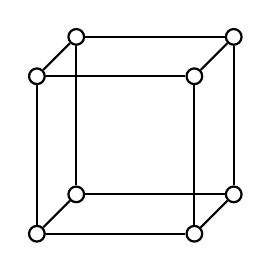
\begin{tikzpicture}
        [nodedecorate/.style={shape=circle,inner sep=2pt,draw,thick},%
          linedecorate/.style={-,thick}]
        %% nodes or vertices
        \foreach \nodename/\x/\y in {1/0/0, 2/2/0, 3/2/2, 4/0/2, 5/0.5/0.5,
          6/2.5/0.5, 7/2.5/2.5, 8/0.5/2.5}
        {
          \node (\nodename) at (\x,\y) [nodedecorate] {};
        }
        %% edges or lines
        \path
        \foreach \startnode/\endnode in {1/2, 2/3, 3/4, 4/1, 5/6, 6/7, 7/8,
          8/5, 1/5, 2/6, 3/7, 4/8}
        {
          (\startnode) edge[linedecorate] node {} (\endnode)
        };
        \end{tikzpicture}

        \caption{The $3$-hypercube graph}
        \label{fig:hypercube}
    \end{figure}
    
    The structure of a graph is determined entirely by its edges, so we get the
    following definition of a graph automorphism.
    \begin{definition}
        A \emph{graph automorphism} is a permutation of the vertices of a graph
        that preserves its edges.  That is, if a graph has vertices $S$ and
        edges $E \subset S \times S$, a permutation $\sigma: S \to S$ is a graph
        automorphism if for every edge $(u, v)$, we have $(\sigma(u), \sigma(v))
        \in E$.  The automorphisms of a graph form a group under composition.
    \end{definition}

    \begin{definition}
        The \emph{hyperoctahedral group} $H_n$ is the automorphism group of the
        $n$-hypercube.
    \end{definition}

\section{A Construction of the Isotypic Decomposition}
    The hypercube graph has a number of nice properties.  In particular, it is
    distance-transitive. 
    \begin{definition}
        A \emph{distance-transitive} graph is a graph such that given any two
        vertices $u_1$ and $v_1$ at distance $d$ and any other two vertices
        $u_2$ and $v_2$ also at distance $d$, there exists some automorphism
        $\sigma$ of the graph with $\sigma(u_1) = u_2$ and $\sigma(v_1) = v_2$.
    \end{definition}
    The fact that the hypercube graph is distance-transitive allows us to
    compute the isotypic decomposition of $L(\xs)$.  Recall that $\xs = \{0,
    1\}^n$ is the set of vertices of the hypercube graph and that the relevant
    group $S_2 \wr S_n$ is the automorphism group of the graph.  Furthermore,
    $L(\xs)$ is a representation of $S_2 \wr S_n$ with an action induced by the
    action on $\xs$.

    The representation $L(\xs)$ for a distance-transitive graph decomposes into
    the eigenspaces of a particular matrix.  
    \begin{definition}
        The \emph{Laplacian matrix} of a graph with vertices $\{v_1, \ldots,
        v_m\}$ is the $m\times m$ matrix $L = (l_{i,j})_{i,j=1}^m$ defined by
        \[
            l_{i,j} = \begin{cases}
                \mathrm{deg}(v_i) & \text{if $i=j$} \\
                -1 & \text{if $i \ne j$ and $v_i$ is adjacent to $v_j$} \\
                0 & \text{otherwise}
            \end{cases}.
        \]
        It is also the difference between the degree matrix and the adjacency
        matrix of the graph.
    \end{definition}
    The Laplacian matrix of the $2$-hypercube graph is show below.
    \[
        \raisebox{-2.75em}{
        \begin{tikzpicture}
          \node (00) at (-1, 1) {00};
          \node (01) at (1, 1) {01};
          \node (10) at (-1, -1) {10};
          \node (11) at (1, -1) {11};
          \foreach \from/\to in {00/01, 01/11, 11/10, 10/00}
            \draw (\from) -- (\to);
        \end{tikzpicture}
        }
        \qquad\longrightarrow\qquad
        \kbordermatrix{
               & 00 & 01 & 10 & 11 \\
            00 &  2 & -1 & -1 &  0 \\
            01 & -1 &  2 &  0 & -1 \\
            10 & -1 &  0 &  2 & -1 \\
            11 &  0 & -1 & -1 &  2 \\
        }
    \]
    Of course, the Laplacian matrix may be viewed as a linear transformation on
    $L(\xs)$.

    The following theorem makes precise the relationship between the Laplacian
    matrix and the isotypic decomposition of $L(\xs)$ in the case of a
    distance-transitive graph.  The following theorem is a close corollary of a result
    by \citeauthor{Sta84}, produced by translating a result for the adjacency
    matrix into a result for the Laplacian matrix.  Because a distance
    transitive graph is regular, the eigenspaces of the Laplacian matrix and of
    the adjacency matrix are the same.  If each vertex has degree $d$, then an
    eigenspace with eigenvalue $\lambda$ with respect to the Laplacian matrix
    has eigenvalue $d - \lambda$ with respect to the adjacency matrix.
    \begin{theorem}[\citet{Sta84}]
        Let $\xs$ be the vertices of a distance transitive graph, and let $G$ be
        the automorphism group of the graph, so that $L(\xs)$, the space of
        complex-valued functions on $\xs$, is a representation of $G$.  Then the
        isotypic decomposition of $L(\xs)$ is multiplicity-free, and is given by
        \[
            L(\xs) = W_{\lambda_1} \oplus \cdots \oplus W_{\lambda_k}
        \]
        where the $\lambda_i$ are distinct eigenvalues of the Laplacian matrix,
        $W_{\lambda_i}$ is the eigenspace corresponding to $\lambda_i$.  In
        particular, the eigenspaces of the Laplacian matrix are irreducible
        representations of $G$.
        \label{thm:dist-trans}
    \end{theorem}

    The eigenspaces for the Laplacian and adjacency matrices of the
    $n$-hypercube graphs have a recursively defined basis.
    \begin{theorem}[\cite{CW06}]
        Let $Q_n$ be the adjacency matrix of the $n$-hypercube graph.  If $v$
        is an eigenvector of $Q_{n-1}$ with eigenvalue $\lambda$, then the
        concatenated vectors $\adel{v_1, \ldots, v_{2^{n-1}},v_1, \ldots,
        v_{2^{n-1}}}$ and $\adel{v_1, \ldots, v_{2^{n-1}}, -v_1, \ldots,
        -v_{2^{n-1}}}$ are eigenvectors of $Q_n$ with eigenvalues $\lambda +1$
        and $\lambda - 1$ respectively.
        \label{thm:eigs}
    \end{theorem}

    \begin{corollary}
        The eigenvalues of the Laplacian matrix of the $n$-hypercube graph are
        $\{0, 2, 4, \ldots, 2n\}$.
        \label{cor:eigs}
    \end{corollary}

    \begin{corollary}
        An eigenbasis of $L(\xs)$ with respect to the Laplacian matrix of the
        $n$-hypercube graph is given by the so-called Walsh functions on $\{0,
        1\}^n$.
        \label{cor:walsh}
    \end{corollary}

    These results given an explicit algorithm to compute the isotypic
    decomposition of $L(\xs)$ for $\xs = \{0, 1\}^n$.

\section{A Parametrization for Binary Log-Linear Models}
    
    We now give a parametrization for $L(\xs)$ in accordance with
    Theorem~\ref{thm:thm}.  We do explicit computations for $n=3$, but the
    construction generalizes.  
    
    From Theorem~\ref{thm:dist-trans} and Corollary~\ref{cor:eigs}, the isotypic
    decomposition of $L(\xs)$ is
    \[
        L(\xs) = W_0 \oplus W_0 \oplus \cdots \oplus W_{2n}
    \]
    where $W_{2j}$ is the eigenspace of the Laplacian matrix with eigenvalue
    $2j$.  From Theorem~\ref{thm:eigs}, the irreducible representations in
    $L(\xs)$ have the following bases.  A function $f: \{0, 1\}^n$ is
    represented as a column vector containing the values of $f$ evaluated on
    each binary string in lexicographic order.
    \[
        W_0 = \adel*{
        \begin{rmatrix}
            1 \\ 1 \\ 1 \\ 1 \\ 1 \\ 1 \\ 1 \\ 1
        \end{rmatrix}
        }
        \qquad
        W_2 = \adel*{
        \begin{rmatrix}
            1 \\ -1 \\ 1 \\ -1 \\ 1 \\ -1 \\ 1 \\ -1
        \end{rmatrix}
        ,
        \begin{rmatrix}
            1 \\ 1 \\ -1 \\ -1 \\ 1 \\ 1 \\ -1 \\ -1
        \end{rmatrix}
        ,
        \begin{rmatrix}
            1 \\ 1 \\ 1 \\ 1 \\ -1 \\ -1 \\ -1 \\ -1
        \end{rmatrix}
        }
    \]
    \[
        W_4 = \adel*{
        \begin{rmatrix}
            1 \\ -1 \\ -1 \\ 1 \\ 1 \\ -1 \\ -1 \\ 1
        \end{rmatrix}
        ,
        \begin{rmatrix}
            1 \\ -1 \\ 1 \\ -1 \\ -1 \\ 1 \\ -1 \\ 1
        \end{rmatrix}
        ,
        \begin{rmatrix}
            1 \\ 1 \\ -1 \\ -1 \\ -1 \\ -1 \\ 1 \\ 1
        \end{rmatrix}
        }
        \qquad
        W_6 = \adel*{
        \begin{rmatrix}
            1 \\ -1 \\ -1 \\ 1 \\ -1 \\ 1 \\ 1 \\ -1
        \end{rmatrix}
        }
        \qquad
    \]

    Let the base point in $\xs$ be $x_0 = 00 \cdots 0$.  Then the stabilizer $K
    = \mathrm{fix}_G(x_0)$ in $S_2 \wr S_n$ is the copy of $S_n$ in $S_2 \wr
    S_n$ that rearranges the bits but does not flip any bit.  Notice that under
    the action of $S_n$, vectors in any one of the above bases are mapped to
    another vector in the basis.  It follows that the sum of the vectors in any
    basis is $K$-invariant.  Thus
    \[
        \begin{rmatrix}
            1 \\ 1 \\ 1 \\ 1 \\ 1 \\ 1 \\ 1 \\ 1
        \end{rmatrix}
        \in W_0,
        \quad
        \begin{rmatrix}
            3 \\ 1 \\ 1 \\ -1 \\ 1 \\ -1 \\ -1 \\ -3
        \end{rmatrix}
        \in W_2,
        \quad
        \begin{rmatrix}
            3 \\ -1 \\ -1 \\ -1 \\ -1 \\ -1 \\ -1 \\ 3
        \end{rmatrix}
        \in W_4,
        \quad
        \text{and }
        \begin{rmatrix}
            1 \\ -1 \\ -1 \\ 1 \\ -1 \\ 1 \\ 1 \\ -1
        \end{rmatrix}
        \in W_6
    \]
    are $K$-invariant vectors.  Under the action of $S_2 \wr S_n$, and
    identifying vectors which are scalar multiples of each other, we get
    the following spanning sets.
    \begin{gather}
        W_0 = \adel*{
        \begin{rmatrix}
            1 \\ 1 \\ 1 \\ 1 \\ 1 \\ 1 \\ 1 \\ 1
        \end{rmatrix}
        }
        \qquad
        W_2 = \adel*{
        \begin{rmatrix}
            3 \\ 1 \\ 1 \\ -1 \\ 1 \\ -1 \\ -1 \\ -3
        \end{rmatrix}
        ,
        \begin{rmatrix}
            1 \\ 3 \\ -1 \\ 1 \\ -1 \\ 1 \\ -3 \\ -1
        \end{rmatrix}
        ,
        \begin{rmatrix}
            1 \\ -1 \\ 3 \\ 1 \\ -1 \\ -3 \\ 1 \\ -1
        \end{rmatrix}
        ,
        \begin{rmatrix}
            1 \\ -1 \\ -1 \\ -3 \\ 3 \\ 1 \\ 1 \\ -1
        \end{rmatrix}
        } 
        \label{eq:spanning}
        \\
        \nonumber
        W_4 = \adel*{
        \begin{rmatrix}
            3 \\ -1 \\ -1 \\ -1 \\ -1 \\ -1 \\ -1 \\ 3 
        \end{rmatrix}
        ,
        \begin{rmatrix}
            -1 \\ 3 \\ -1 \\ -1 \\ -1 \\ -1 \\ 3 \\ -1
        \end{rmatrix}
        ,
        \begin{rmatrix}
            -1 \\ -1 \\ 3 \\ -1 \\ -1 \\ 3 \\ -1 \\ -1
        \end{rmatrix}
        ,
        \begin{rmatrix}
            -1 \\ -1 \\ -1 \\ 3 \\ 3 \\ -1 \\ -1 \\ -1
        \end{rmatrix}
        }
        \qquad
        W_6 = \adel*{
        \begin{rmatrix}
            1 \\ -1 \\ -1 \\ 1 \\ -1 \\ 1 \\ 1 \\ -1
        \end{rmatrix}
        }
        \qquad
    \end{gather}

\section{Other Parametrizations}

    Some of the motivation for identifying another spanning set comes from the
    paper by \citet{SPEC}.  In that paper, the authors consider a number of
    spanning sets for $L(\xs)$ where $\xs = \{0, 1\}^n$.  With these spanning
    sets, the authors fit log-linear models with $L_1$ regularization to binary
    data, as described in Section~\ref{sec:regularization} of this paper.

    The spanning sets considered in the paper by \citet{SPEC}, along with their
    names for them, are as follows.

    The \emph{full parametrization} contains functions of the form
    \[
        f_{S, g}(b_1 \cdots b_n) = \begin{cases}
            1 & \text{when $b_i = g(i)$ for all $i \in S$} \\
            0 & \text{otherwise}
        \end{cases}
    \]
    where $S$ is any subset of $\{1, \ldots, n\}$ and $g$ is any function $S \to
    \{0, 1\}^{|S|}$.  This parametrization contains $3^n$ functions.

    The \emph{canonical parametrization} contains functions of the form
    \[
        f_S(b_1 \cdots b_n) = \begin{cases}
            1 & \text{when $b_i = 1$ for all $i \in S$} \\
            0 & \text{otherwise}
        \end{cases}.
    \]
    for all $S \subset \{1, \ldots, n\}$.  This parametrization contains $2^n$
    functions.

    The \emph{spectral parametrization} contains the $2^n$ Walsh functions on
    $\{0, 1\}^n$ as in Theorem~\ref{thm:eigs} and Corollary~\ref{cor:walsh}.

    Our spanning set as in Equation~\ref{eq:spanning} shares with the spectral
    parametrization the properties that the set is invariant (as a set) under
    the action of $S_2 \wr S_n$ and that appropriate subsets of the set generate
    the irreducible representations in $L(\xs)$.  Additionally, our spanning set
    seems well-suited to weighting single points heavily while only selecting a
    few subspaces.

\chapter{Conclusion}

\section{Future Directions}

\section{For Further Reading}


\appendix


% \nocitep{*}


\backmatter

\bibliographystyle{hmcmath}
\bibliography{thesis}

%\printindex


\end{document}




